\documentclass{beamer}


\graphicspath{{figures/}}
\usepackage{tikz}
\usetikzlibrary{positioning, arrows}
%\usetheme{boxes}
\usepackage[utf8]{inputenc}
\usepackage{amsmath}
\usepackage{amsthm}
\usepackage{hyperref}
\usepackage[font=tiny]{caption}
\usepackage{booktabs}
\usepackage{natbib}
\bibliographystyle{plainnat}
\usecolortheme{crane}

\definecolor{orange}{RGB}{232, 86, 15}
\definecolor{blue}{RGB}{14, 159, 232}
\definecolor{blueblue}{RGB}{50, 90, 160}
\definecolor{yellow}{RGB}{232, 187, 14} 
\definecolor{red}{RGB}{232, 14, 59}

\hypersetup{
  colorlinks=true,
  linkcolor=cyan,
  urlcolor=cyan,
  citecolor=purple
}
\newtheorem{deff}{Definición}
%Information to be included in the title page:
\institute[]{}

\setbeamercolor{title}{bg=blueblue, fg=white}
\setbeamercolor{subttile}{bg=blueblue, fg=white}
\setbeamercolor{frametitle}{bg=blueblue, fg=white}
\setbeamercolor{block title}{bg=blue, fg=white}
\setbeamercolor{block title alerted}{bg=red, fg=white}
\setbeamercolor{block title example}{bg=yellow, fg=white}
\setbeamercolor{footline}{bg=gray, fg=white}

\beamertemplatenavigationsymbolsempty

\newcommand{\indep}{\perp \!\!\! \perp}
\title{(Casual) Causality Course 2025 \\ Session 1}
\author{Gherardo Varando}
\date{25 March 2025}
\begin{document}

\begin{frame}
\maketitle
\end{frame}

\begin{frame}{(Casual) Causality Course 2025}

	\begin{block}{Intructors}
	  \begin{itemize}
	    \item Gherardo \url{gherardo.varando@uv.es}
	    \item Emiliano \url{emiliano.diaz@uv.es} 
	    \item Vassilis \url{vasileios.sitokonstantinou@uv.es}
	  \end{itemize}
	\end{block}
	
	\begin{block}{Schedule} 
         \begin{itemize}
	   \item \textbf{week 1, Tuesday} Intro and causal inference (GV)
	   \item \textbf{week 1, Thursday} Causal inference and robustness (GV)    
	   \item \textbf{week 2, Tuesday} Causal Discovery (ED)
	   \item \textbf{week 2, Thursday} Causal Discovery (ED)
	   \item \textbf{week 3} Intensive weeek with group projects! 
	 \end{itemize}
	\end{block}


\end{frame}


\begin{frame}{Learning outcomes} 

  \begin{columns}
    \begin{column}{0.5\textwidth}
  \begin{itemize}[<+-|alert@+>]
    \item Understand the fundamental
          goals and problems of causal methods  
    \item Familiarize with the vocabulary, definitions and basic concepts of causality
    \item Understand the fundamentals behind basic methodologies in
          causal inference and causal discovery
	\item How causal methods and tools are relevant in ML?
  \end{itemize}
    \end{column}
    \begin{column}{0.5\textwidth}
      \only<1>{
	\begin{figure}
	  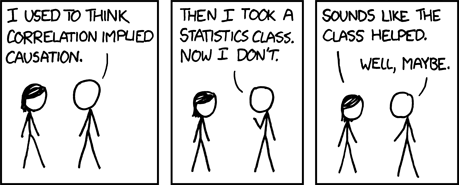
\includegraphics[width=5cm]{correlation}
	  \caption{xkcd (CC BY-NC 2.5) \url{https://xkcd.com/552}}
	\end{figure}
      }
\only<2>{
	\begin{figure}
	  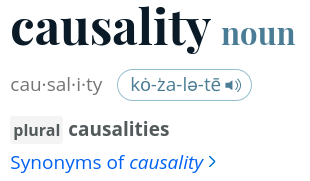
\includegraphics[width=5cm]{causality_noun}
	  \caption{\url{https://www.merriam-webster.com/dictionary/causality}}
	\end{figure}
      }
\only<3>{
	\begin{figure}
	  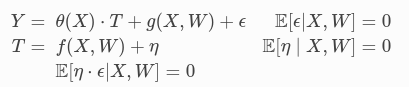
\includegraphics[width=5cm]{dml}
	  \caption{\url{https://econml.azurewebsites.net}}
	\end{figure}
      }
 \only<4>{
	\begin{figure}
	  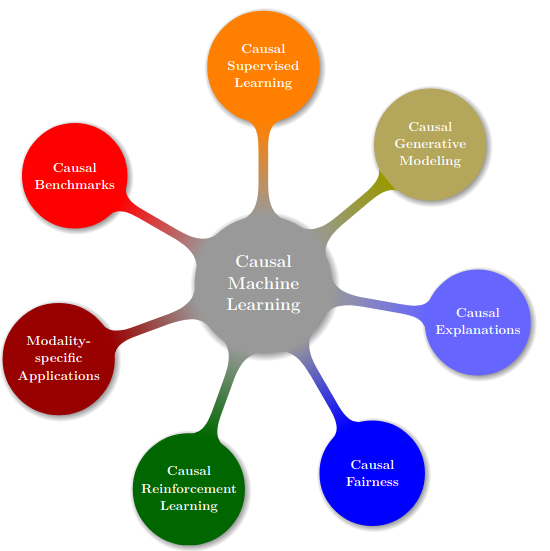
\includegraphics[width=5cm]{causal_ml}
	  \caption{From \cite{kaddour2022causalmachinelearningsurvey}}
	\end{figure}
      }
    \end{column}
  \end{columns}
\end{frame}

\begin{frame}{Content week 1}
  \begin{itemize}
    \item \textbf{Session 1} Tue 25/03
      \begin{itemize}
	\item[Part I] \textbf{Intro to causality and causal methods} \\ 
	  \only<2>{motivation, causal questions, what is causality? \\
		      experiments, interventions and counterfactuals \\ 
		      structural causal models and graphs}
         \item[Part II] \textbf{Basics of causal inference} \\
	     \only<2>{causal effect, randomized experiments  \\
	              observational studies, identifiability conditions \\
		      graphical representation, confounding, selection bias \\
		      random variability and measurement error 
	   } 
      \end{itemize}
\vfill
    \item \textbf{Session 2} Thu 27/03
      \begin{itemize}
	\item[Part I] Causal inference methods
	\item[Part II] Robustness to interventions  
      \end{itemize}
  \end{itemize}
\end{frame}

\begin{frame}{Basic references}
  \begin{itemize}
    \item \href{https://mitpress.mit.edu/9780262037310/elements-of-causal-inference/}{Elements of causal inference} \citep{peters2017elements} [EC] 
    \item \href{https://miguelhernan.org/whatifbook}{Causal Inference: What If} \citep{hernan2025causal} [Wif]
    \item All of Statistics \citep{wasserman2013all} [AoS] 
  \end{itemize}

  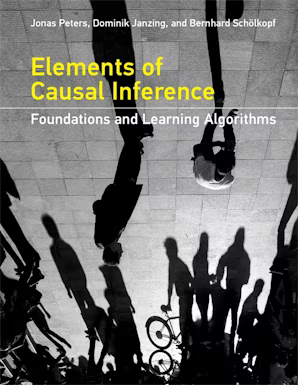
\includegraphics[width = 2 cm]{elements}
  
\includegraphics[width = 2 cm]{whatif}
  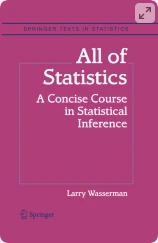
\includegraphics[width = 2 cm]{all}
\end{frame}


\begin{frame}{}


  \begin{columns}
    \begin{column}{0.8\textwidth}
  \begin{quote}
Felix qui potuit rerum cognoscere
causas \dots \\
    \hfill \small \textnormal{Publius Vergilius Maro \\ \hfill Georgica \href{https://www.poetryintranslation.com/PITBR/Latin/VirgilGeorgicsII.php}{Book Two}}
  \end{quote}
      \onslide<2>{
	\centering
	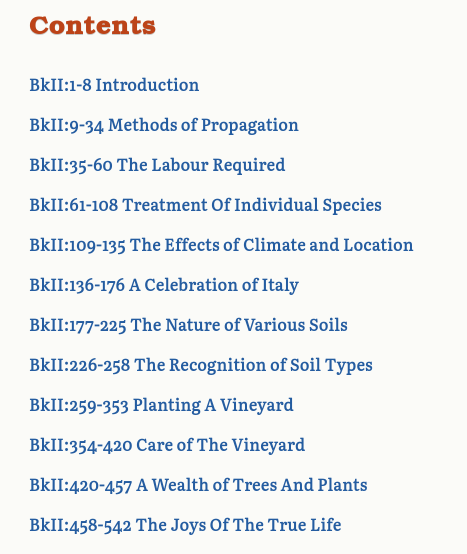
\includegraphics[scale=0.3]{book2index}
      }
    \end{column}
    \begin{column}{0.4\textwidth}
      \begin{figure}
	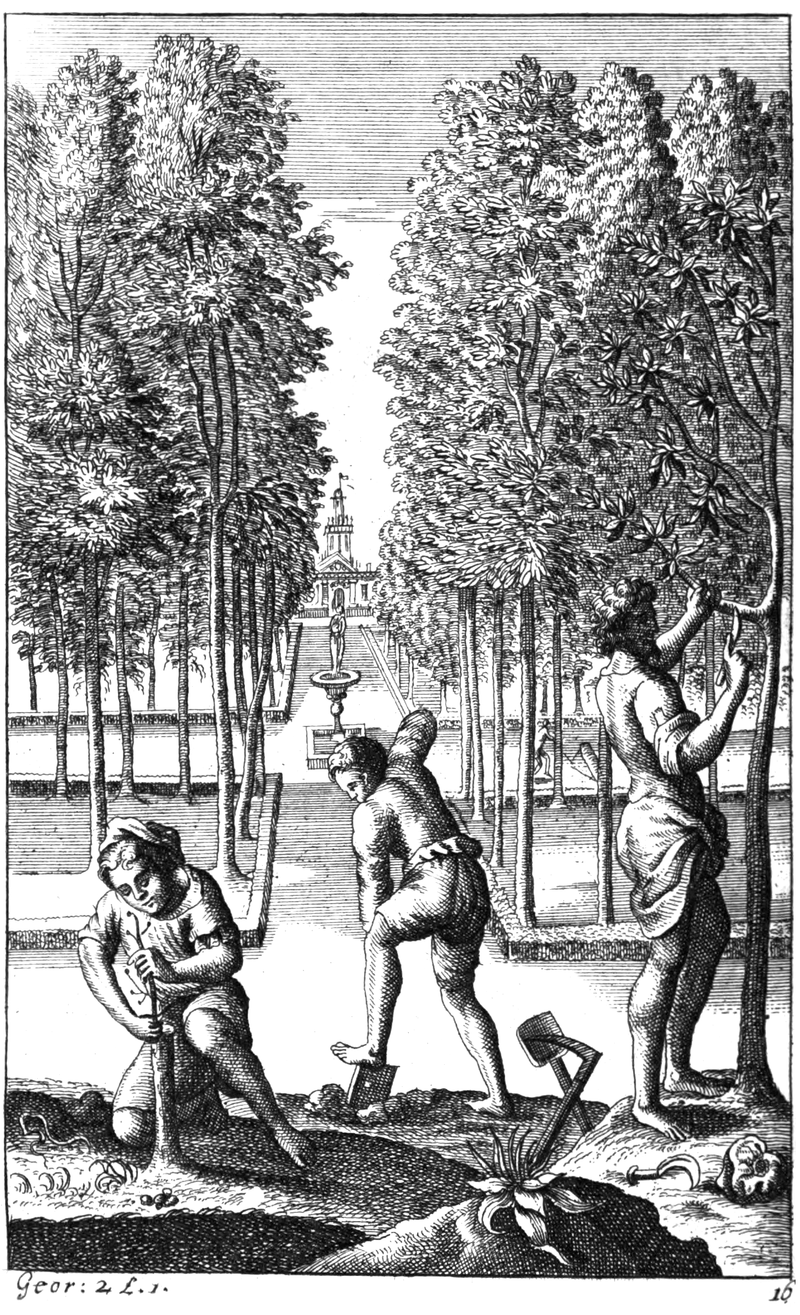
\includegraphics[scale=0.18]{book2}
	\caption{By Michael van der Gucht - \href{https://commons.wikimedia.org/w/index.php?curid=88226096}{Public Domain}}
      \end{figure}
    \end{column}
  \end{columns}
\end{frame}

\begin{frame}{What is causality?}
  \begin{columns}
    \begin{column}{0.7\textwidth}
  %\begin{center}
  %  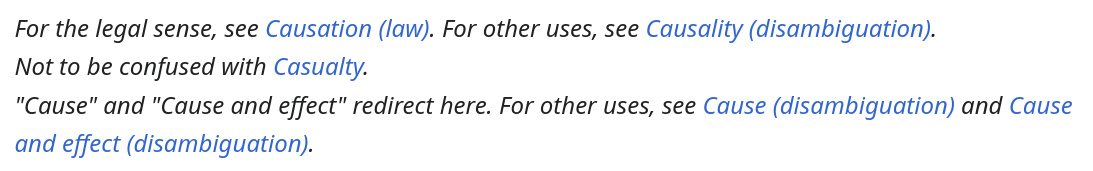
\includegraphics[width=0.95\textwidth]{Causality-Wikipedia}
  %\end{center}
  \begin{itemize}
    \item Causality in Law  \url{https://en.wikipedia.org/wiki/Causation_(law)} \\
      \href{https://www.youtube.com/watch?v=XiCOmhdkM80&list=PLqMxKp2ot-3vDaLyaAZNgt8ijj6n0l460}{Causation|Low of Tort playlist on youtube, first 3 videos}  
    \item Causality in Physics \\
       \url{https://en.wikipedia.org/wiki/Causality_(physics)}  \\
       \url{https://www.youtube.com/watch?v=eG_eHDDMgCs} \\
       \cite{rovelli2022causationrootedthermodynamics}  
  \end{itemize}
  \end{column}
    \begin{column}{0.3\textwidth}
       \begin{figure}
	 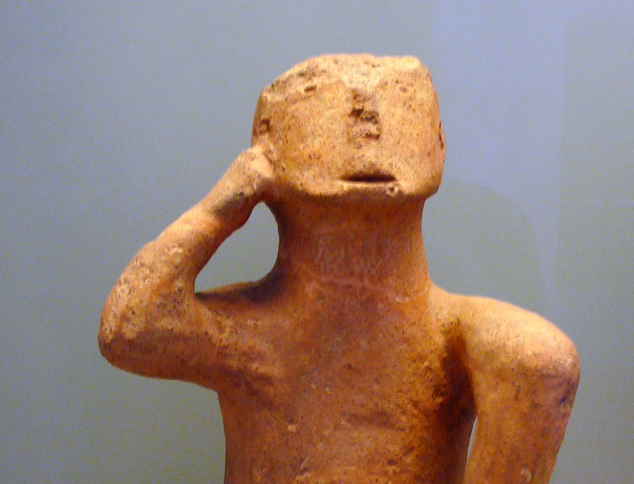
\includegraphics[width=3cm]{thinker1}
	 \caption{Karditsa Thinker at the National Archaeological Museum, Athens} 
       \end{figure}
       \vfill
    \onslide<2->{
      \begin{itemize}
	  \tiny
	\item Work in groups and briefly discuss causality in physics or law 
	      \textbf{[15 min]}, choose a speaker 
	    \item  The two speakers present the main ideas \textbf{[5 min]} (whiteboard, slides)
      \end{itemize}
    }
    \end{column}
  \end{columns}
\end{frame}


\begin{frame}{Non-causal questions ... still important!!}
  
\includegraphics[width=0.45\textwidth]{scientist}
  
\includegraphics[width=0.45\textwidth]{QR0}
\end{frame}

\begin{frame}{Non-causal questions ... still important!!}
  \begin{columns}
    \begin{column}{0.5\textwidth}
      \begin{itemize}[<+-|alert@+>]
	\item Estimate the tree diameters or age in a forest \citep{west2021tamm} 
	\item Counts the number of trees in the desert
	  \citep[\href{https://www.nature.com/articles/s41586-020-2824-5}{unexpectedly high}][]{brandt2020unexpectedly} 
	\item Cloud detection \citep{aybar2024onboard} 
	\item Describing patterns of wood density \citep{yang2024} 
      \end{itemize}
    \end{column}
    \begin{column}{0.5\textwidth}
      \only<1>{
	\begin{figure}
	  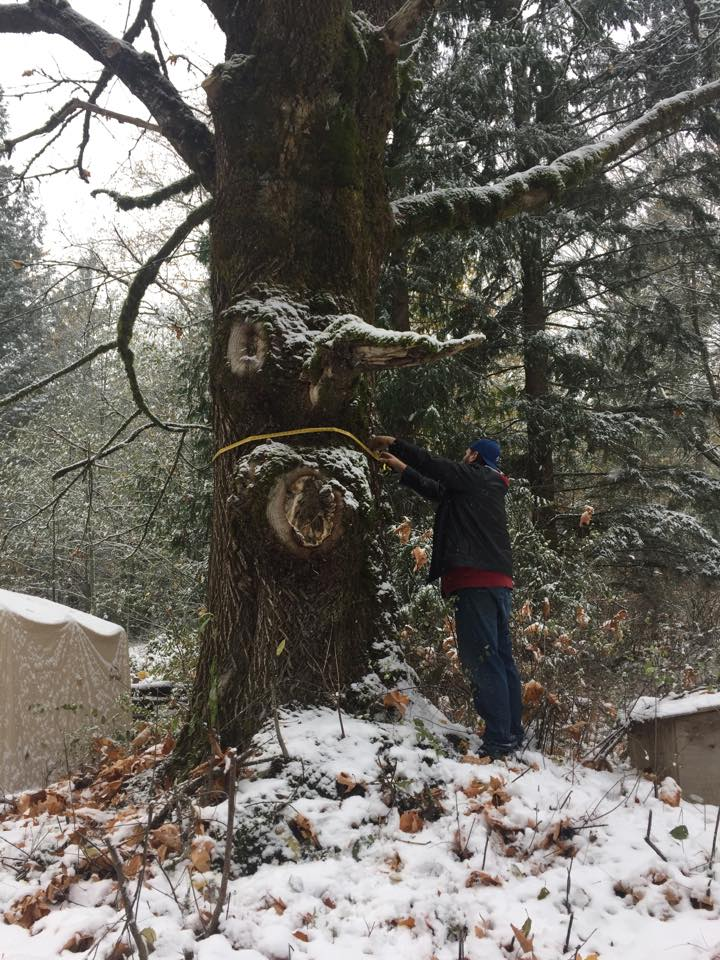
\includegraphics[width=4cm]{tree-meas}
	  \caption{From \url{https://theforestguild.com/estimating-the-age-of-trees/}}
	\end{figure}
      }
      \only<2>{
	\begin{figure}
	  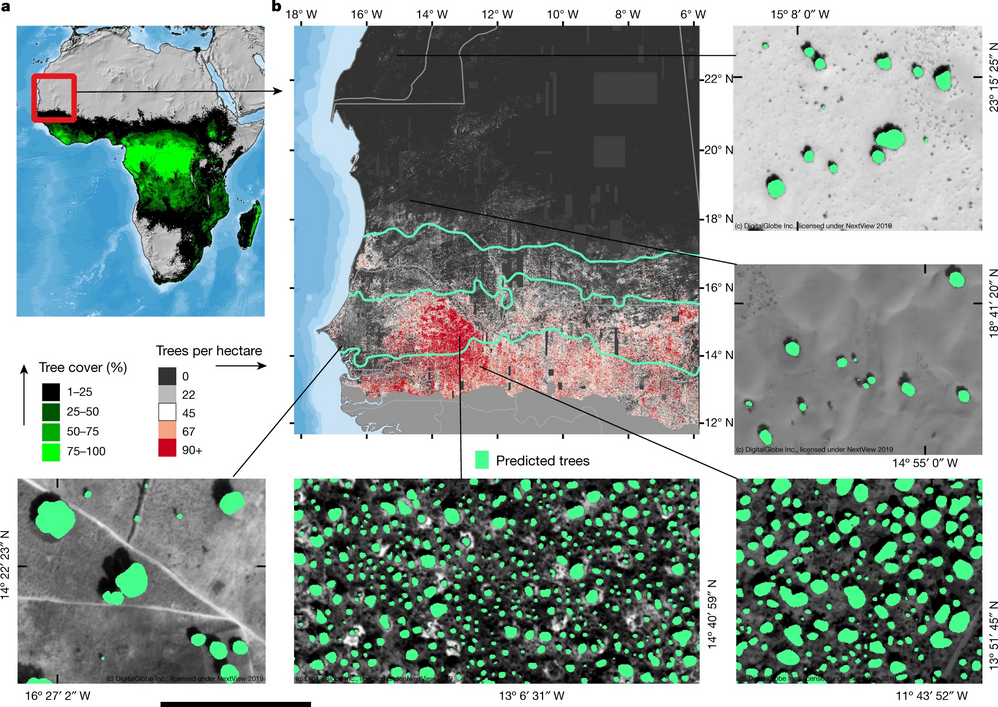
\includegraphics[width=6cm]{tree-desert}
	  \caption{From \cite{brandt2020unexpectedly} \href{https://www.nature.com/articles/s41586-020-2824-5}{paper}}
	\end{figure}
      }
      \only<3>{
	\begin{figure}
	  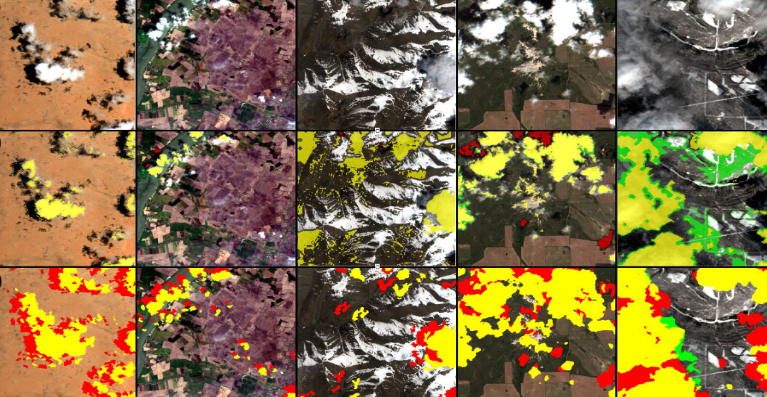
\includegraphics[width=6cm]{cloud}
	  \caption{From \cite{aybar2024onboard} \href{https://events.ecmwf.int/event/304/contributions/3629/attachments/2126/3769/ECMWF-ESA-WS_Garicia-Acciarini.pdf}{poster}} 
	\end{figure}
      }
      \only<4>{
	\begin{figure}
	  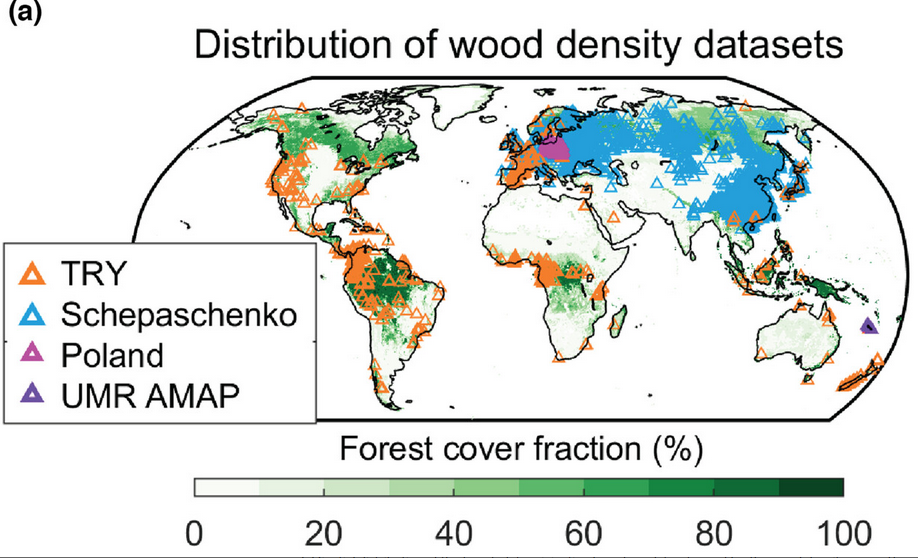
\includegraphics[width=6cm]{wood_density}
	  \caption{From \cite{yang2024} \href{https://onlinelibrary.wiley.com/doi/10.1111/gcb.17224}{paper}} 
	\end{figure}
      }
    \end{column}
  \end{columns}

\end{frame}


\begin{frame}{Causal questions}
  
\includegraphics[width=0.45\textwidth]{QR0}
  
\includegraphics[width=0.45\textwidth]{scientistthink}
\end{frame}

\begin{frame}{Causal questions}
  \begin{columns}
    \begin{column}{0.5\textwidth}
      \begin{itemize}[<+-|alert@+>]
	\item How droughts affect yields 
	\item Evaluate agricultural practice \citep{tsoumas2023evaluating, Giannarakis_2022_CVPR} 
	\item How does armed conflict influence tropical forest loss? \citep{Christiansen03042022} 
	\item Estimate the effect of ENSO on vegetation \citep{le2023increased} 
      \end{itemize}
    \end{column}
    \begin{column}{0.5\textwidth}
      \only<1>{
	\begin{figure}
	  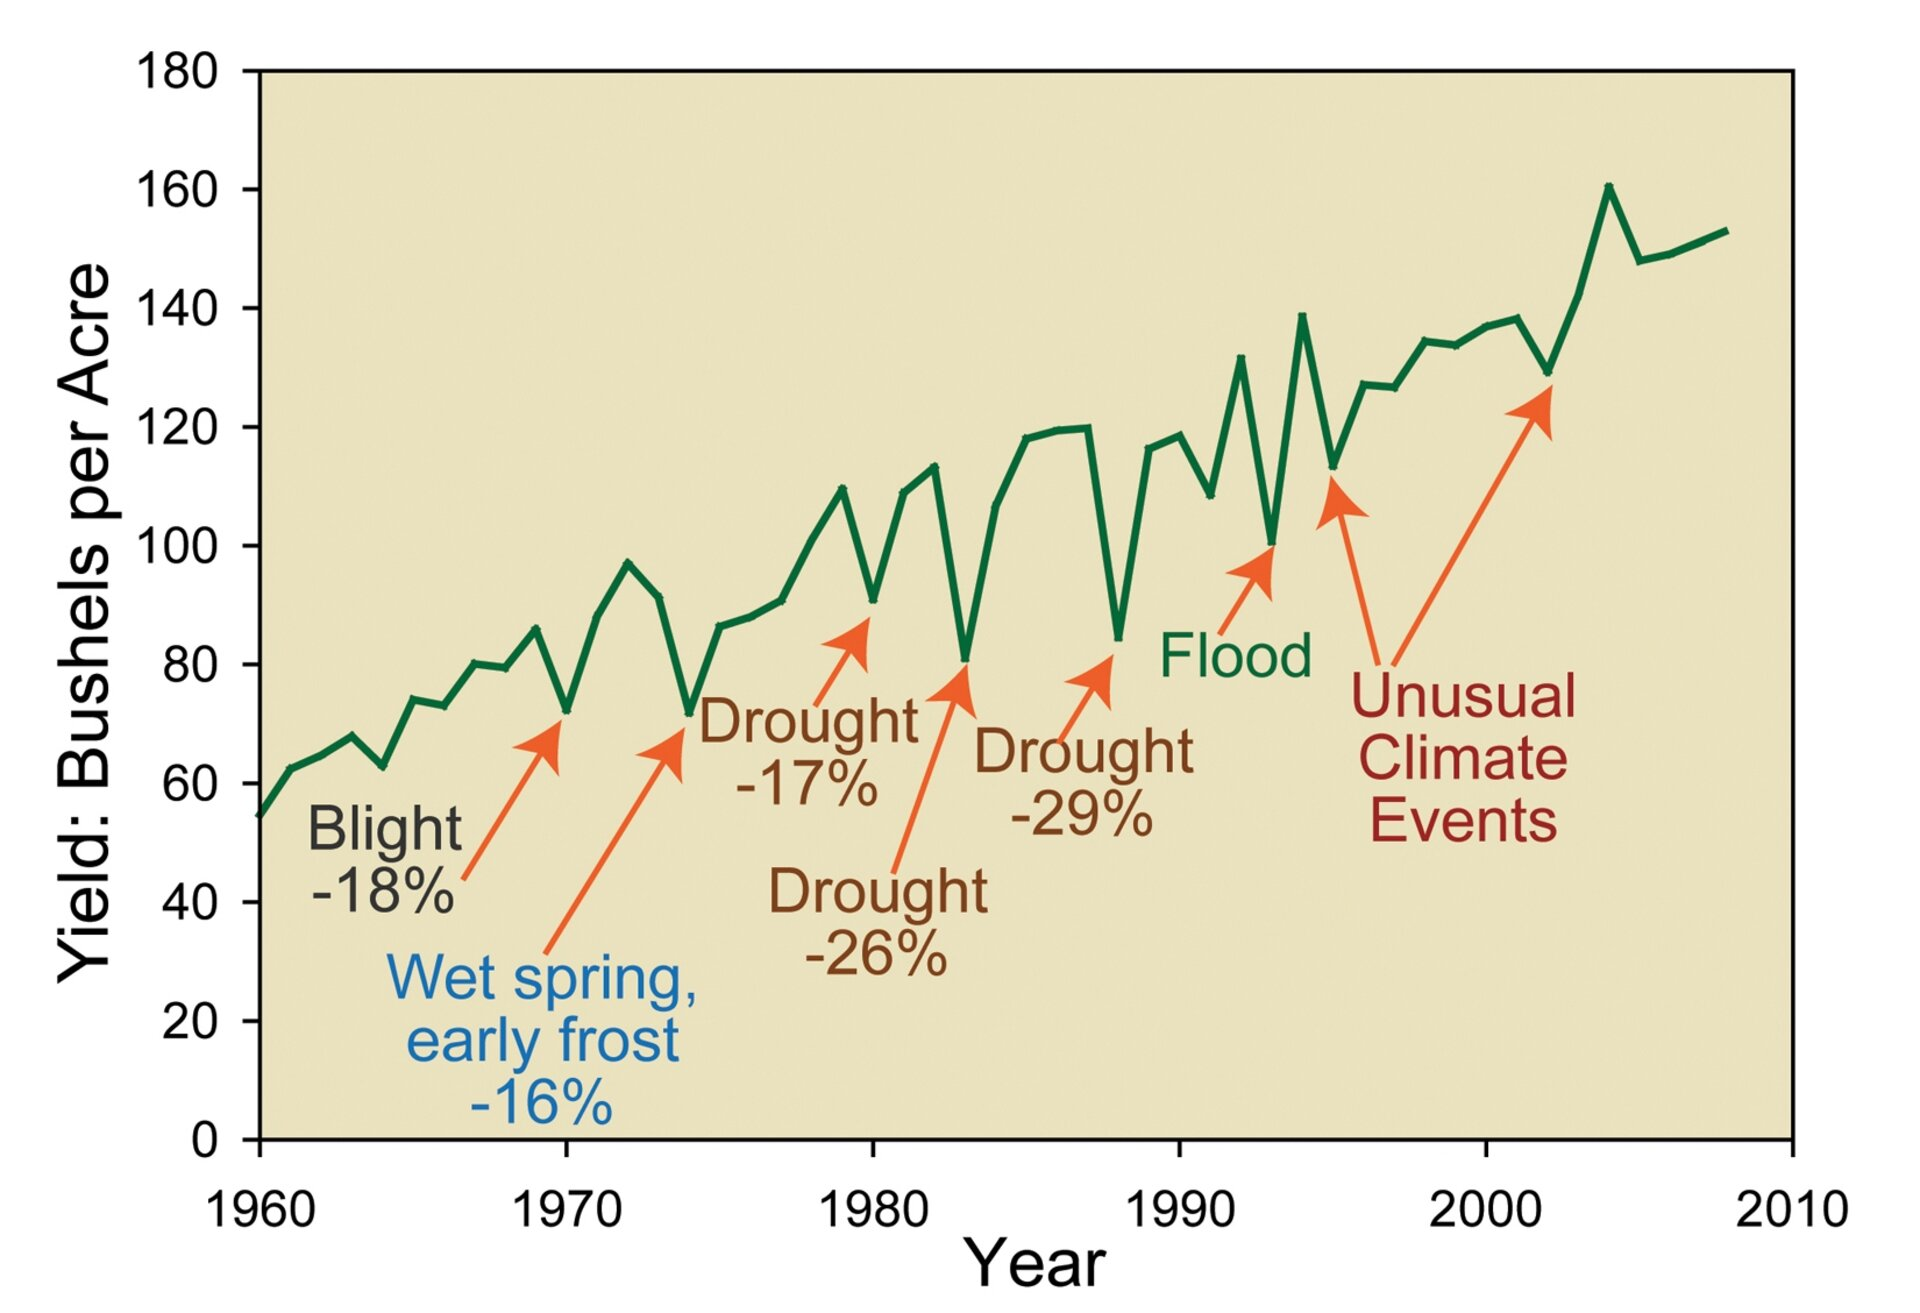
\includegraphics[width=6cm]{effect_drought}
	  \caption{credit USDA FAS, from \href{https://www.esa.int/ESA_Multimedia/Images/2014/05/Effect_of_drought_on_corn_yields}{ESA Website} (ESA Standard
Licence)}
	\end{figure}
      }
      \only<2>{
	\begin{figure}
	  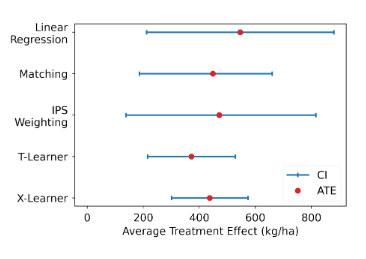
\includegraphics[width=6cm]{agri_effect}
	  \caption{From \cite{tsoumas2023evaluating}}
	\end{figure}
      }
      \only<3>{
	\begin{figure}
	  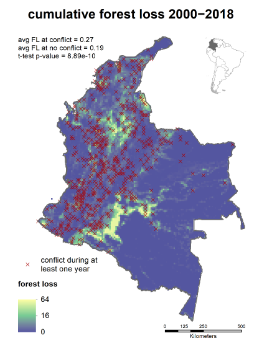
\includegraphics[width=4cm]{forest_loss}
	  \caption{From \cite{Christiansen03042022}} 
	\end{figure}
      }
      \only<4>{
	\begin{figure}
	  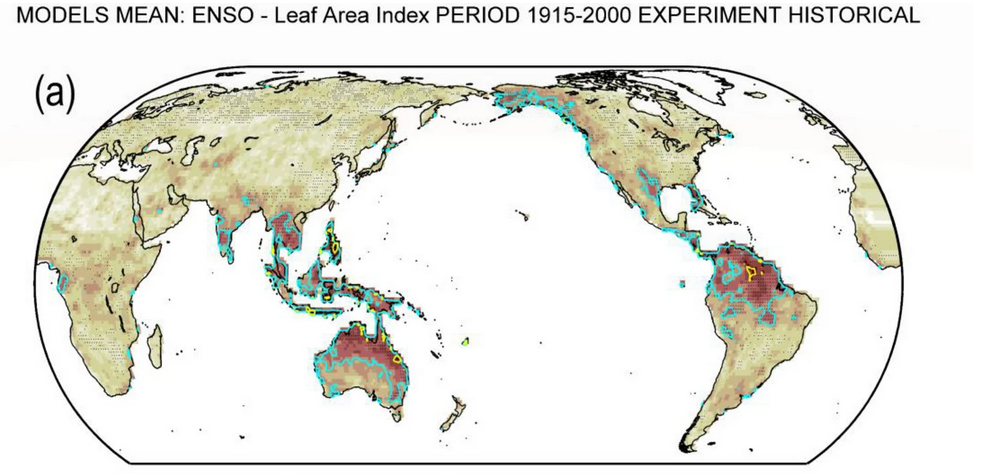
\includegraphics[width=7cm]{enso_veg}
	  \caption{From \cite{le2023increased}} 
	\end{figure}
      }
    \end{column}
  \end{columns}

\end{frame}


\begin{frame}{Probabilistic causation}

  \begin{block}{\citep[][AoS, Chapter 16]{wasserman2013all}}
    \begin{quote}
	Roughly speaking, the statement `` $X$ causes $Y$'' means that 
	changing the value of $X$ will change the distribution of $Y$.
      \end{quote}
  \end{block}
  \begin{itemize}
    \item<2-> How to make the previous \emph{definition} precise and operative? 
    \item<3-> What does it mean \text{changing the value} of $X$? 
    \item<4-> various solutions are possible, we will see two possibilities:
      \textbf{Structural Causal Models (SCM)} and the \textbf{Potential Outcome framework}
  \end{itemize}
\end{frame}

\begin{frame}{Structural Causal Models}
	\begin{block}{Definition \citep{peters2017elements}}
 A SCM over variables $X_1, \ldots, X_p$ with noise variables $\varepsilon_1, \ldots, \varepsilon_p$ is 
	 a collection of \textbf{structural assignments}: 
	   \[ X_i =  f_i(X_{pa(i)}, \varepsilon_i) \]
	   where $\varepsilon_i$ are assumed jointly independent and $f_i$ are fixed deterministic functions.  
	 \end{block}
	 \begin{itemize}
		 \item $X_{pa(i)}$ are called the parents or the \textbf{direct causes} of $X_i$
		 \item we say $X_i$ is a direct effect of its direct causes 
		 \item we assume the associated graph $G$ to be a DAG 
	 \end{itemize}
\end{frame}

\begin{frame}
  \begin{example}
    \begin{columns}
      \begin{column}{0.45\textwidth}
    A simple SCM for variables 
    \begin{itemize}
      \item $Y$ cotton yield  
      \item $SM$ soil moisture on sowing 
      \item $TS$ temperature on sowing 
      \item $T$ sowing is performed on optimal day (1)  or not (0)  
    \end{itemize}
      \end{column}
      \begin{column}{0.45\textwidth}
    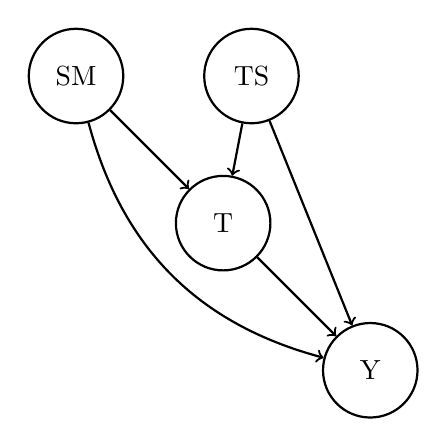
\begin{tikzpicture}[
    roundnode/.style={circle, draw=black, thick, minimum size=1.2cm},
    directed/.style={->, thick}
]

% Nodes
\node[roundnode] (SM) {SM};
\node[roundnode, right=of SM] (TS) {TS};
\node[roundnode, below right=of SM] (T) {T};
\node[roundnode, below right=of T] (Y) {Y};

% Edges
\draw[directed] (SM) -- (T);
\draw[directed] (TS) -- (T);
\draw[directed, bend right=30] (SM) to (Y);
\draw[directed] (TS) -- (Y);
\draw[directed] (T) -- (Y);

\end{tikzpicture}

      \end{column}
    \end{columns}

    \begin{align*}
    SM &= 0.3 + \epsilon_{SM} \\
    TS &= 25 + \epsilon_{TS} \\
      T  &= \mathbf{1}_{>0} \left( 1.2 + 0.8 SM - 0.05 TS + \epsilon_T > 0 \right) \\
      Y  &= \max\{0, \, 2.5 + 1.5 SM - 0.7 TS + 2.0 T + \epsilon_Y\} 
\end{align*}
  \end{example}
\end{frame}


\begin{frame}{SCMs as statistical models}
\begin{block}{}
      Every SCM define a unique distribution over the considered variables.  
    \end{block}
  \begin{columns}
\begin{column}{0.5\textwidth}
    \begin{itemize}
      \item<2-> How? \ldots 
      \item<3-> We can sample from the SCM following \textbf{a topological order of the DAG} 
      \item<4-> If we can generate observations, we implicitly defined a distribution 
    \end{itemize}
\end{column}
\begin{column}{0.5\textwidth}
  \begin{figure}
  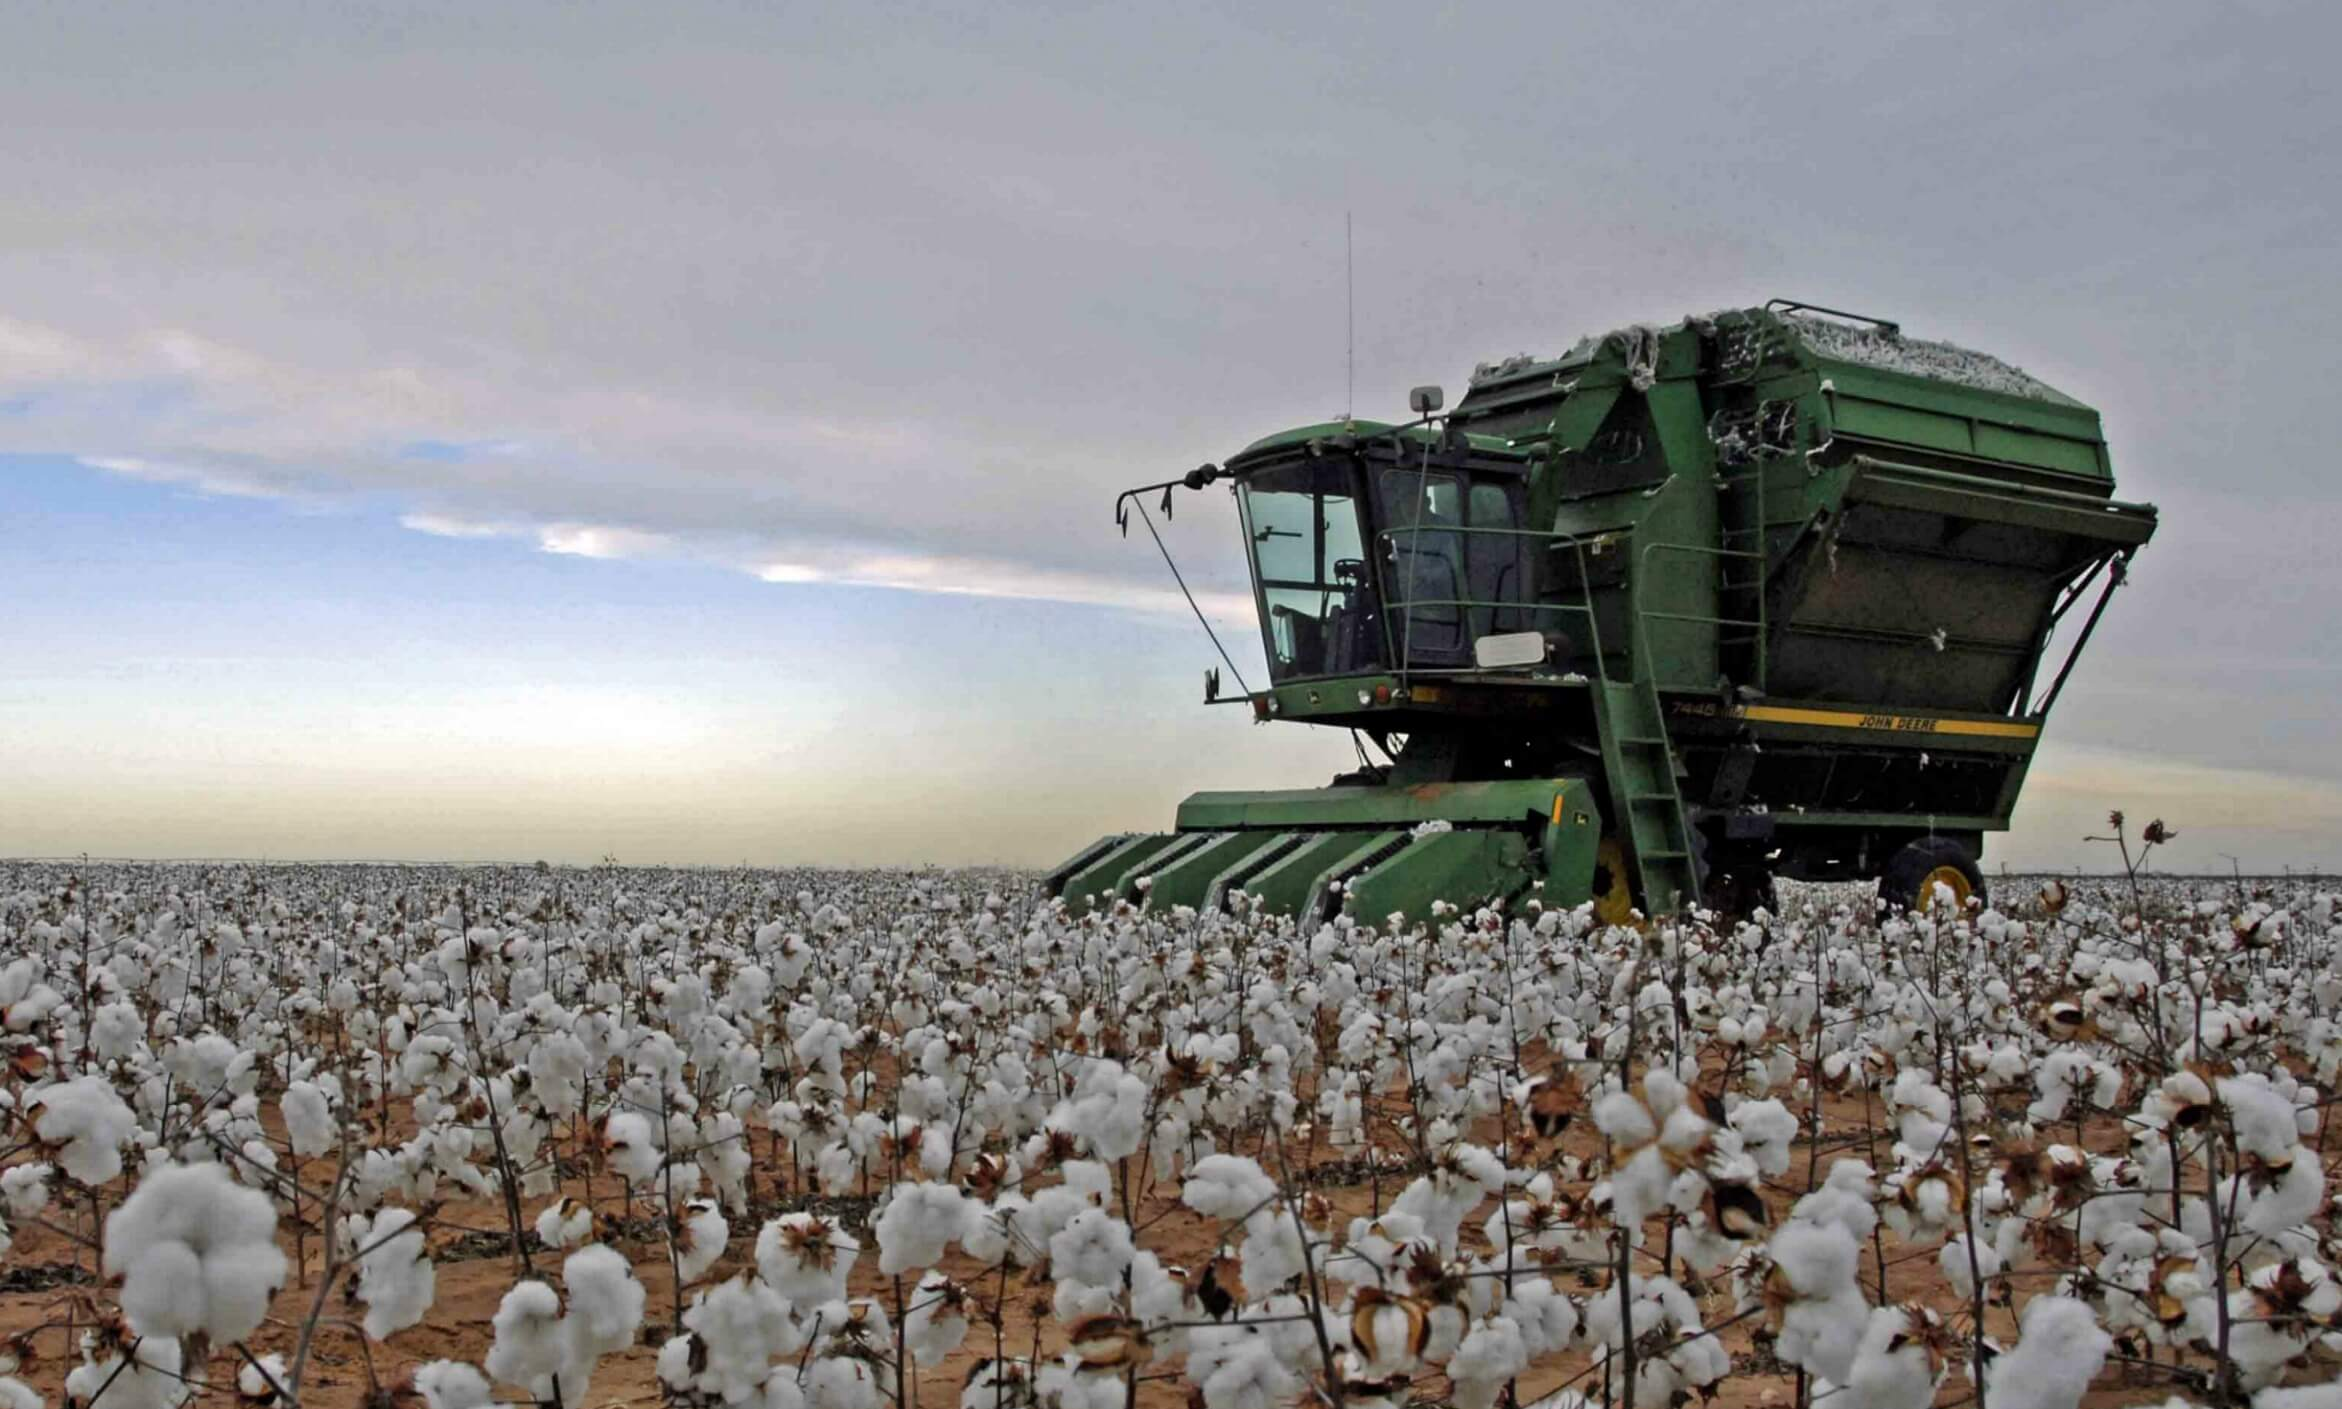
\includegraphics[width=\textwidth]{cotton-picker}
    \caption{From \url{https://www.quilting-in-america.com/cotton-cultivation-process.html}}
  \end{figure}
\end{column}
  \end{columns}
\end{frame}



\begin{frame}{SCMs can model interventions or experiments}
\begin{block}{}
  We define an experiment, or intervention when
  we \textbf{replace one or several of the structural assignments}
to obtain a new SCM
    \end{block}
  \begin{columns}
\begin{column}{0.5\textwidth}
    \begin{itemize}
      \item<2-> The interventional distribution under this change is the new
entailed probability distribution defined by the new SCM 
      \item<3-> We indicate probabilities under interventions with e.g.  
	         $P( Y | \operatorname{do}(T = 1))$  
    \end{itemize}
\end{column}
\begin{column}{0.5\textwidth}
  \begin{figure}
  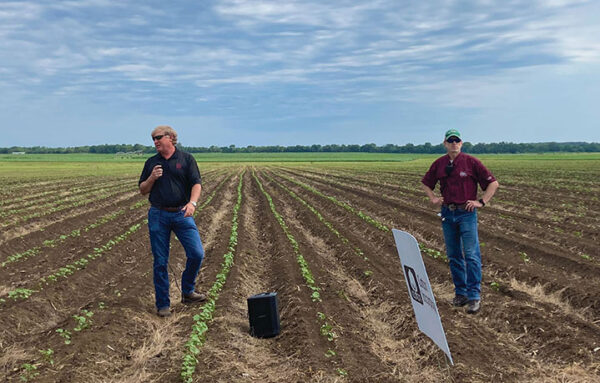
\includegraphics[width=\textwidth]{cotton-exp}
    \caption{From \url{https://www.cottonfarming.com/feature-story/field-day-highlights/}}
  \end{figure}
\end{column}
  \end{columns}
\end{frame}

\begin{frame}
  \begin{definition}[Total causal effect \citet{peters2017elements}] 
We say there is a \textbf{total causal effect} from $T$ to $Y$  if (and only if)
		 there exist $\tilde{N}$ such that 
			\[ T \not \indep Y \text{ in } P^{do(T = \tilde{N})}  \]
  \end{definition}

  \begin{itemize}[<+-|alert@+>]
    \item How we intuitive interpret the definition ?   
    \item If there is no direct path between $T$ and $Y$ then there is no total causal effect 
    \item Sometimes there is a direct path but no total causal effect 
  \end{itemize}
\end{frame}


\begin{frame}{With SCM we can reason about counterfactuals}
\begin{block}{}
  We define an experiment, or intervention when
  we \textbf{replace one or several of the structural assignments}
to obtain a new SCM
    \end{block}
  \begin{columns}
\begin{column}{0.5\textwidth}
  \begin{itemize}

    \item<1-> Given some observed state/event,what would have happened if ... ? 
    \item<2-> Counterfactual statements can be seen as intervention/do-statements in
			a counterfactual SCM which is obtained from an initial SCM by replacing the
			noise distribution with $P(\varepsilon | X = x)$
    \end{itemize}
\end{column}
\begin{column}{0.5\textwidth}
  \begin{figure}
  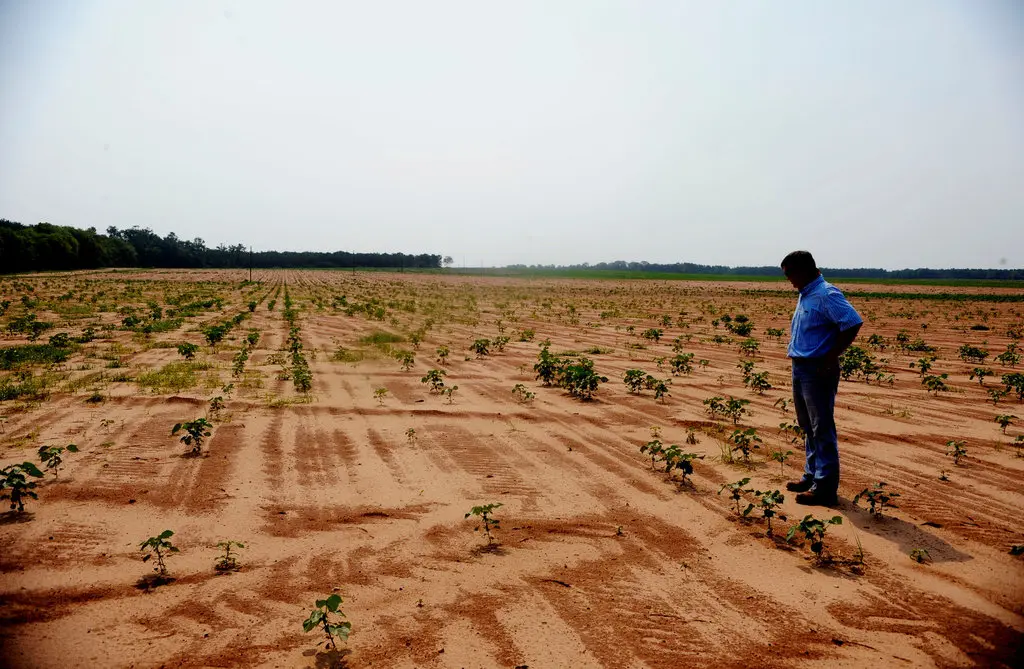
\includegraphics[width=\textwidth]{cotton-drought}
    \caption{From \url{https://www.nytimes.com/2011/07/12/us/12drought.html}}
  \end{figure}
\end{column}
  \end{columns}
\end{frame}


\begin{frame}{Counterfactuals in SCM}
Counterfactuals are  different from interventions since we are not just doing an experiment,
      but rather imagining interventions for alternative \emph{worlds}, that is
      alternative ways the system could have evolved but conditioning on everything
      else being the same
	\begin{itemize}
	  \item SCMs allow the computation of counterfactual probabilities

	  \item SCM can induce same observational and interventional distribution (Causal BN)
	    but different counterfactuals (see example in \cite{peters2017elements}) 
	\end{itemize}

\end{frame}

\begin{frame}{Pearl Causal Hierarchy (PCH) }
  From \cite{bareinboim2022pearl}
	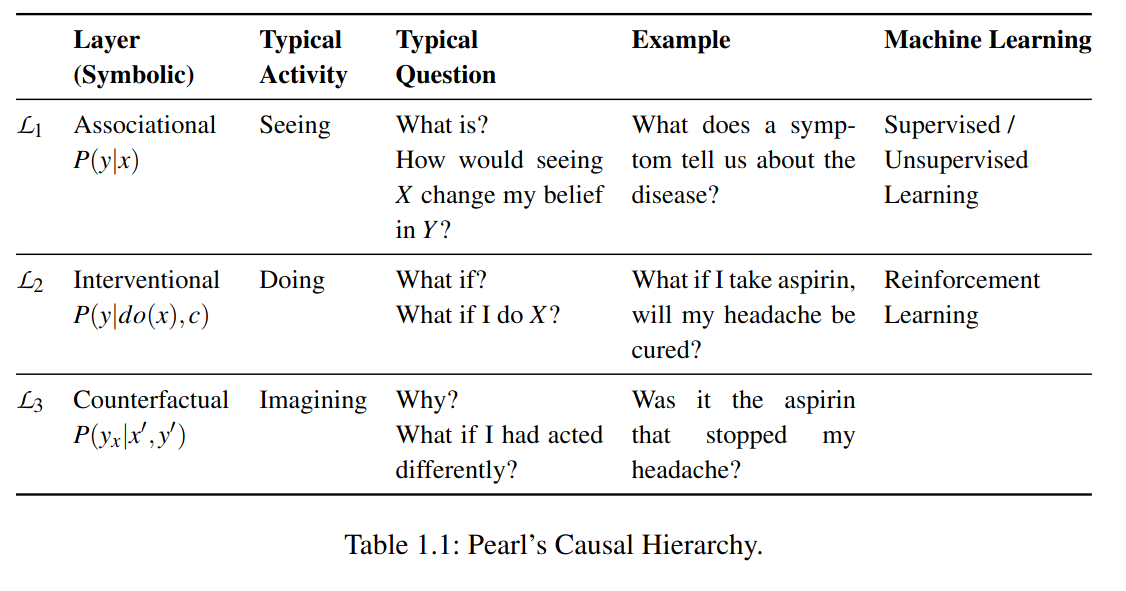
\includegraphics[scale=0.3]{PCH}
\end{frame}

\begin{frame}{On the concept of \emph{Harm}} 
  \begin{itemize}
    \item \cite{sarvet2023perspective}  interventionalist vs contrefactual  
    \item \cite{mueller2024perspective} response 
  \end{itemize}
\end{frame}


\begin{frame}{Personalized decision making}
  \begin{itemize}
    \item \cite{mueller2023personalized} 
    \item \cite{tian2000probabilities} 
  \end{itemize}
\end{frame}

\begin{frame}{Potential outcomes - Counterfactual model}
  \begin{columns}
    \begin{column}{0.5\textwidth}
  \cite{hernan2025causal} \cite{wasserman2013all}  
  \begin{itemize}
    \item consider a binary \textbf{treatment variable} $A$
      (1: forest management practice (thinning, controlled burns,...) , 0: wild/uncontrolled forest)
    \item and a binary \textbf{outcome} $Y$ (1: burned area, 0: not burned)
    \item $A,Y$ are random variables that take possible different values for each individual
  \end{itemize}
  \vfill
    \end{column}
    \begin{column}{0.5\textwidth}
      \begin{figure}
      \includegraphics[width = \textwidth]{burn}
	\caption{From \url{https://www.kunc.org/2024-03-15/long-term-study-finds-combination-of-prescribed-burns-thinning-effective-at-reducing-wildfire-risk}} 
      \end{figure}
    \end{column}
  \end{columns}

\end{frame}


\begin{frame}{Potential outcomes - Counterfactual model}
  \begin{columns}
    \begin{column}{0.5\textwidth}
  \cite{hernan2025causal} \cite{wasserman2013all}  
  \begin{itemize}
    \item<1-> denote with the outcome variable that would have been observed under treatment $a=1$, and similarly $Y^{a=0}$
    \item<2-> $Y^{a=1}$ and $Y^{a=0}$ are called \textbf{potential outcomes} or \textbf{counterfactual outcomes}
    \item<3-> for each individual, only one of the potential outcomes
      is actually observed/factual.
      \[ Y = Y^{a=A}  \quad \text{(consistency equation)} \]
  \end{itemize}
    \end{column}
    \begin{column}{0.5\textwidth}
      \begin{figure}
      \includegraphics[width = \textwidth]{burn}
	\caption{From \url{https://www.kunc.org/2024-03-15/long-term-study-finds-combination-of-prescribed-burns-thinning-effective-at-reducing-wildfire-risk}} 
      \end{figure}
    \end{column}
  \end{columns}

\end{frame}


\begin{frame}{Causal effects}
  \begin{definition}{Average causal effects}
    An average causal effect of treatment $A$ on outcome $Y$ is present if
    \[ P(Y^{a=1} = 1) \neq   P(Y^{a=0} = 1) \]
    or equivalently (for binary outcomes)
    \[ \mathbb{E}[Y^{a=1}] \neq \mathbb{E}[Y^{a=0}] \]
  \end{definition}
  \begin{itemize}
    \item<2-> in practice we need to \textbf{measure} causal effects
    \item<3-> {causal risk difference} $P(Y^{a=1} = 1) - P(Y^{a=0} = 1)$
    \item<4-> {causal risk ratio} $\frac{P(Y^{a=1} = 1)}{P(Y^{a=0} = 1)}$
    \item<5-> {causal odds ratio} $\frac{P(Y^{a=1} = 1) / P(Y^{a=1} = 0) }{P(Y^{a=0} = 1) / P(Y^{a=0} = 0)}$
  \end{itemize}
\end{frame}



\begin{frame}{Randomized experiments}
  \begin{columns}

    \begin{column}{0.5\textwidth}
  \begin{itemize}
    \item<1-> We collect data following a randomized control study:
      for each individual (forest unit/patch)  we flip a coin and we assign the treatment variable
      to be $a=1$ if heads and $a=0$ if tails.
    \item<2-> We then collect the outcome variable $Y$ (e.g. burned or not after 1 year) for all individuals in
      the study
  \end{itemize}
    \end{column}
    \begin{column}{0.5\textwidth}
     \begin{figure}
       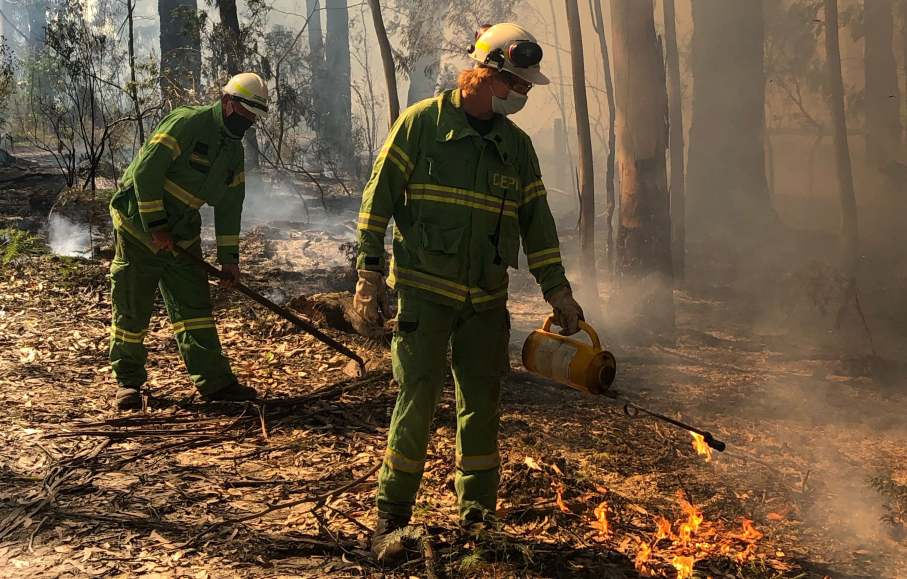
\includegraphics[width = \textwidth]{crew}
     \end{figure}
    \end{column}
  \end{columns}
\end{frame}

\begin{frame}{Randomized experiments}
  \begin{columns}

    \begin{column}{0.5\textwidth}
  \begin{itemize}
    \item<1-> assume no problem with the study, everybody is following instruction and
      there are no measurements problems (\emph{ideal randomized experiment})
    \item<2-> can we say something about the causal effect of $A$ on $Y$ ?
    \item<3-> yes! we can compute the average causal effect ... formally because there
      is \textbf{exchangeability} between the treated ($A=1$) and untreated ($A=0$) groups
  \end{itemize}
    \end{column}
    \begin{column}{0.5\textwidth}
     \begin{figure}
       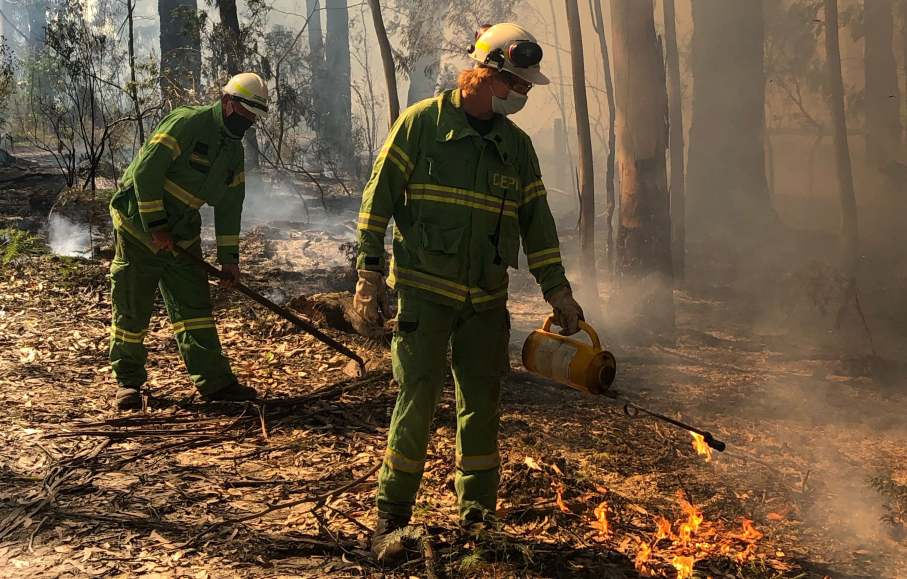
\includegraphics[width = \textwidth]{crew}
     \end{figure}
    \end{column}
  \end{columns}
\end{frame}

\begin{frame}
	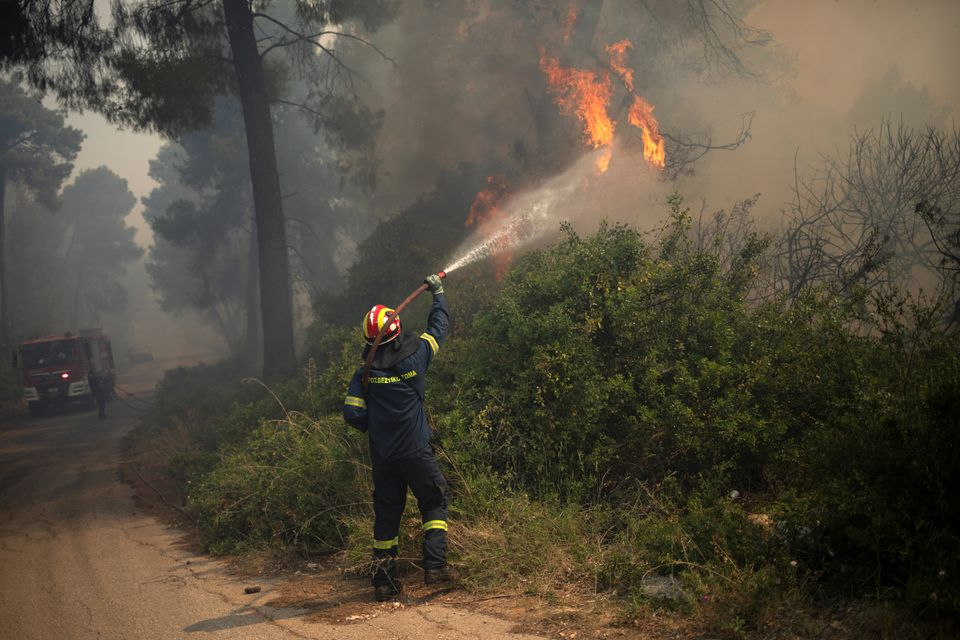
\includegraphics[scale=0.2]{fire}

	\textbf{New problem: the firefighters do not like your randomized study}
	they say that it is too dangerous not to manage some patches at all, and that some
	areas have a too high fire risk to be left completely untreated
\end{frame}

\begin{frame}{Conditional randomized experiments}
  \begin{itemize}
    \item<1-> Assume we have now a covariate $L$, measured before treatment was assigned
      (e.g. risk of fire: low, medium, high)
    \item<2-> We divide the population into strata based on the levels of $L$
      and we perform randomization with different probabilities in each stratum
      (e.g. 0.8 for low fire risk, 0.5 for medium fire risk, and 0.2 for high fire risk)
    \item<3-> In each stratum, we have exchangeability and we can compute
      average treatment effects
    \item<4-> this is called \emph{stratification}
    \item<5-> moreover we say that this procedure ensure \textbf{conditional exchangeability}                          $Y^a \indep A | L$
  \end{itemize}
\end{frame}

\begin{frame}{Computing ATE from conditionally randomized data}
	\begin{itemize}
		\item<1-> From the data collected with a conditionally randomized experiment we can compute
			the ATE in all population.
		\item<2-> \textbf{Standardization} consists in computing the
			marginal counterfactual risk
			as the weighted average of the stratum-specific risk.
			\[ P(Y^a = 1) = \sum P(Y^a = 1| L = l)P(L = l) \]
		\item<3-> \textbf{Inverse Probability Weighting} is an alternative, but equivalent,
			procedure to compute $P(Y^a = 1)$ by weighting each individual sample
			by $w_l = 1 / P(A = a|L = l)$ and then we compute $P(Y^a = 1) = \sum w_l P(Y | A= a, L = l)$
	\end{itemize}
\end{frame}



\begin{frame}{Observational studies}
	Sometimes is unethical, too expensive or simply impossible to conduct experiments, so we are left only with observational data, what can we do? (e.g. we just collect historical
	data on forest management practice  and burned areas)
	\begin{itemize}
		\item<2-> Problems: confounding variables (e.g. forest are controlled more when we expect to
			have high risk of fire, patients are treated with more invasive/effective treatments when doctors thinks the case is more serious, \ldots)
		\item<3->  still under certain conditions and assumptions we can identify the
			causal effect
		\item<4-> this conditions 
		  \emph{assure that the observational study can be used
			somehow as a randomized trial}
	\end{itemize}
\end{frame}

\begin{frame}{Identifiability conditions}
  \begin{enumerate}
    \item<1-> \textbf{Exchangeability} the conditional probability
      of receiving every value of treatment, though
      not decided by the investigators, depends only on measured covariates $L$
    \item<2-> \textbf{Positivity} the probability of
      receiving every value of treatment conditional on $L$ is
      greater than zero, i.e., positive
    \item<3-> \textbf{Consistency} the values of treatment under comparison
      correspond to well-defined interventions that,
      in turn, correspond to the versions of treatment in the data
  \end{enumerate}
  \only<4>{If we can assume this three conditions we can use the techniques such as IPW or standardization to compute ATE from observational data}
\end{frame}

\begin{frame}{Effect modification}

  \begin{itemize}
    \item We say that $V$ is a modifier of the effect of $A$ on $Y$
      when the average causal effect of $A$ on $Y$ varies across levels of $V$
    \item \textbf{Stratification} or \textbf{matching} can be used to identify effect modification
    \item<2-> To construct our matched population we replaced the treated in the 
      population by a subset of the treated in which the matching factor $L$ had the
      same distribution as that in the untreated.
    \item<3-> they require exchangeability and positivity
    \item<4-> Standardization (or IPW), stratification and matching measure different
      causal effects: Average effects in the entire population, conditional causal effects (startification) and usually causal effects in the treated and untreated for matching
  \end{itemize}

\end{frame}



\begin{frame}[allowframebreaks]{Bibliography}
  \tiny
\bibliography{biblio}
\end{frame}

\end{document}


